\documentclass[11pt, oneside]{article}   	% use "amsart" instead of "article" for AMSLaTeX format
\usepackage{geometry}                		% See geometry.pdf to learn the layout options. There are lots.
\usepackage{listings}
\usepackage{color}
\usepackage{framed}
\usepackage{url}
\geometry{letterpaper}                   		% ... or a4paper or a5paper or ... 
%\geometry{landscape}                		% Activate for for rotated page geometry
%\usepackage[parfill]{parskip}    		% Activate to begin paragraphs with an empty line rather than an indent
\usepackage{graphicx}				% Use pdf, png, jpg, or eps� with pdflatex; use eps in DVI mode
								% TeX will automatically convert eps --> pdf in pdflatex		
\usepackage{amssymb}
\usepackage{float}

%\FrameSep0pt

\restylefloat{figure}
%\setlength{\intextsep}{1.8ex}
\setlength{\parindent}{0pt}

\definecolor{dkgreen}{rgb}{0,0.6,0}
\definecolor{gray}{rgb}{0.5,0.5,0.5}
\definecolor{mauve}{rgb}{0.58,0,0.82}
 
\lstset{ %
  language=Java,                			% the language of the code
  basicstyle=\footnotesize,           		% the size of the fonts that are used for the code
  %numbers=,                   			% where to put the line-numbers
  %numberstyle=\tiny\color{gray},  		% the style that is used for the line-numbers
  %stepnumber=1,                   			% the step between two line-numbers. If it's 1, each line 
                                  				% will be numbered
  numbersep=5pt,                  			% how far the line-numbers are from the code
  backgroundcolor=\color{white},      	% choose the background color. You must add \usepackage{color}
  showspaces=false,               			% show spaces adding particular underscores
  showstringspaces=false,        		 % underline spaces within strings
  showtabs=false,                			 % show tabs within strings adding particular underscores
  %frame=single,                   			% adds a frame around the code
  rulecolor=\color{black},        		% if not set, the frame-color may be changed on line-breaks within not-black text (e.g. commens (green here))
  tabsize=4,                      			% sets default tabsize to 2 spaces
  captionpos=b,                   			% sets the caption-position to bottom
  breaklines=true,                			% sets automatic line breaking
  breakatwhitespace=false,        		% sets if automatic breaks should only happen at whitespace
  title=\lstname,                   			% show the filename of files included with \lstinputlisting;
                                  				% also try caption instead of title
  keywordstyle=\color{blue},          		% keyword style
  commentstyle=\color{dkgreen},       	% comment style
  stringstyle=\color{mauve},         		% string literal style
  escapeinside={\%*}{*)},            		% if you want to add LaTeX within your code
  morekeywords={*,...}               		% if you want to add more keywords to the set
}

\title{COMS4507 - Mental Poker Application}
\author{Ben Evans and Emile Victor}
%\date{}							% Activate to display a given date or no date

\begin{document}
\maketitle

\section{Abstract}

The Mental Poker application created provides a decentralised method of poker hand distribution over the internet for a 7-card Texas Holdem game. The application makes use of RSA encryption and signing of individual cards to prevent cheating, and is able to abort a game if any cheating is detected.\\
					
All communication is directed through a scalable publish/subscribe server which acts somewhat like a proxy passing messages from user to user. All of the underlying communication, cryptography and game decision making components are performed in a background thread, and the results are displayed on screen. All functionality relating to game joining and hosting is also visualised on a GUI, which communicates to a back-end application running the program logic.\\
					
While the application is quite effective at what it does, there remain a couple of vulnerabilities which are inherent in the design choices made during its construction. They are outlined in Section \ref{sec:securityConcerns} in detail.

\section {Purpose}

The Mental Poker algorithm is an algorithm which allows poker cards to be dealt without a centralized third party. It allows each player to ensure that every other player is not cheating, which is incredibly necessary in internet play. \\

The intent of the Mental Poker application was to provide a safe and reliable way of dealing hands over the internet, without having to rely on a central server for any gameplay elements. All elements barring the cryptography and communications subsystems mostly follow the description of the system described in the week 3 lecture notes relating to Mental Poker. However, the communications system utilises a central scalable Elvin server.\\

This program, once complete could be extended to provide truly P2P poker play, without the need for a centralized message passing server. It was determined however that there is some need for a centralised server when dealing with the banning of players. Both the centralised message passing and P2P approaches allows each player in the swarm to trust their money in said game, as they themselves are able to guarantee that every player has not cheated.

\section{Implementation}

The Mental Poker application consists of 5109 lines of Java code, all of which are available at \url{https://github.com/BennyEvans/CardEncryption}. The application utilises multi-threading through Swingworkers, the Swing GUI framework, the UQ-designed Elvin notification subsystem and a fairly large amount of homespun encryption code.\\ 

The application is essentially a terminal application which performs gameplay and game search/joining, which has been modified to allow for GUI hooks. It uses multiple methods to communicate to and from the GUI, and to ensure a responsive and quick GUI at all times.\\

The implementation uses multiple encryption and decryption steps to assure security. As an example, if two players wanted to play a game of Poker they would need some way of securely shuffling the deck. If they don't wish to rely on a third party then the Mental Poker algorithm could be used. This is how the dealing of cards would be done:\\

Player one first encrypts and shuffles the deck. Player one then sends the shuffled and encrypted deck to player two who also encrypts and shuffles the deck. Player two then sends the doubly shuffled and encrypted deck back to player one. At this point everyone has shuffled and encrypted the deck and player one and two have no clue as to which card is which. Player one then chooses two random cards for themselves and two random cards for player two and sends player two's cards to player two. Player one and player two then both encrypt their encrypted hands again with different keys. They then both ask each other to decrypt their doubly encrypted hands. After this, player one and player two are both left with their encrypted hands that are encrypted twice by themselves with different keys (the reason for this is explained in Sections \ref{sec:encryption} and \ref{sec:validation}). After decrypting their own cards, each player has securely received their hand.

\subsection{Communications Subsystem}
\label{sec:comsubsys}				

Elvin is utilised for all inter-player communication. Elvin is a high-performance, scalable publish/subscribe system. Elvin was chosen because it was thought to be the best of both a centralised and decentralised poker system. By using a centralised communications server, additional security for players is added as players are not directly connected to each other, nor do they know one another's IP or location. Players only rely on a third party (the Elvin server) for message passing. The Elvin server has no input on gameplay so players can be assured they are not being scammed by a biased third party card dealer. The other advantage of using a central communications server is that logging can occur at the server and cheaters or rogue users can be denied service. This can be done by IP and can effectively block the cheater from all games that are being played using that communications server.\\

The implementation utilises the UQ Elvin server, and transmits pre-encrypted text strings and binary representing cards for each user, along with game information and hosting information. Hosts simply enter a loop sending out notifications every few sections that they have a game available. Players wishing to join listen for these messages and receive a list of available hosts to join. When they choose to join, they are put into a lobby where they wait until all slots are filled. The host is able to watch while slots are filled up in their GUI.

\subsection{Encryption}
\label{sec:encryption}

\begin{figure}[H]
	\caption{RSA variables used in the generation of the encryption and decryption keys.}
	\vspace{0.2cm} 
  	\centering
	\begin{framed}
		$n=pq$\\$\phi=(p-1)(q-1)$
	\end{framed}
	\vspace{-0.45cm} 
	\label{fig:rsavars}
\end{figure}

Encryption is performed using commutative RSA. The aim of commutative RSA is to allow encryption and decryption to happen in an arbitrary order and thus allow users to decrypt cards in a different order than that in which they were encrypted. Commutative RSA is the key to Mental Poker. The implementation utilises the BouncyCastle Cryptography library to aid in encryption and decryption.\\

Commutative RSA works by sharing common p and q primes. From this n and $\phi$ (see Figure \ref{fig:rsavars}) can be calculated. The encryption key is randomly generated and needs to be relatively prime to $\phi$ and smaller than $\phi$. In the application implementation, the encryption key e is chosen as a prime number so if $\phi$ mod( e ) is not equal to zero then e is relatively prime to $\phi$.  The decryption key d is then calculated as the modular inverse of e, ie. find d where $ed = 1 mod ( \phi)$. In commutative RSA both e and d are kept private.\\

Figure \ref{fig:code} shows the Java code for key generation in the application implementation. The code makes use of the BigInteger library to deal with the massive numbers needed for RSA encryption to be effective. 

\begin{figure}[H]
\caption{Key Generation.}
\begin{framed}
\begin{lstlisting}
private void genKeys() throws NoSuchAlgorithmException,
			InvalidKeySpecException {
		BigInteger tmp;
		BigInteger testRes;
		while (true) {
 			/* Generate a prime and make sure it is coprime to on */
			tmp = genPrime(KEY_SIZE);
			/* on = (p-1) * (q-1). Computed in a different function */
			testRes = on.divideAndRemainder(tmp)[1];
			if (testRes.compareTo(BigInteger.ZERO) != 0) {
				e = tmp;
				d = e.modInverse(on);
				return;
			}
		}
	}
\end{lstlisting}
\vspace{-0.45cm} 
\end{framed}
\vspace{-0.45cm} 
\label{fig:code}
\end{figure}

Each user encrypts their hand twice for added protection against the replay of cards in further decryption stages. Their hand is encrypted with their original encryption key used to encrypt the deck, and once receiving their hand, this hand is encrypted again with another purely private (no one can request to decrypt against this key) encryption key with the same p and q as the first. The reason behind this will be further discussed in section \ref{sec:validation} when dealing with the community cards decryption round.

\subsection{Validation}
\label{sec:validation}

Validation is used in the implementation of anti-cheating measures. There are two forms of validation used in the implementation of Mental Poker.

\subsubsection{Card Validation}

Card validation is performed in two places in the implementation. Validating the community cards is the first of this type of validation. Validating the community cards is performed using the following algorithm:

\begin{itemize}
\renewcommand{\labelitemi}{$\bullet$}
\item The game host chooses 5 random cards (not in play) from the fully encrypted deck (encrypted with every game users’ key).
\item The game host broadcasts these 5 cards for everyone to receive.
\item Every player in the game then asks every other player to decrypt the community cards (in order). Explained further below.
\item Once everyone has decrypted the cards, the game host broadcasts their version of the plaintext community cards.
\item Each user then compares their decrypted versions of the community cards with the game hosts’ plaintext version. If any user disagrees they call cheat and the game is closed.
\end{itemize}

The community card decryption round also has some added protection to prevent against a rogue user asking another user to decrypt that users own hand without them knowing. The implementation provides a secure method to prevent this from happening.This is done by comparing decryption requests. In the case of a two player game each user simply compares a decryption request with the original fully encrypted community cards. In the case of a game with more than two players it becomes more complex. The way the implementation deals with this problem is by comparing the decryption requests of users who haven't been the recipient of a decryption round (are yet to decrypt cards).\\

The easiest way to explain this is with an example. Figure \ref{fig:com} shows an example of the community cards decryption rounds in a four player game. In the first round, users 1, 2 and 3 all ask the host (user 4) to decrypt the community cards. User 4 then compares the decryption requests of users 1, 2, 3 and the encrypted community cards they have. If any of the requests differ from one another, cheat is called and the game is ended. In the second round, users 1, 2 and 4 ask user 3 to decrypt the community cards. User 3 then compares the requests of user 1 and 2 with their version of the encrypted community cards. Again, if they differ, cheat is called and the game is ended. User 3 doesn't compare user 4’s request because user 4 has already been the recipient of a decryption round and it is therefore expected that user 4’s request will be different (it will have user 4’s encryption still on it because each user will decrypt their own encryption as the last step). In the third round users 1, 3 and 4 all ask user 2 to decrypt the community cards. In this round, user 2 only compares their version of the encrypted community cards with user 1’s request as user 3 and user 4 have already been the recipient of a decryption round. In the final decryption round, users 2, 3 and 4 ask user 1 to decrypt the community cards. User 1 does not compare any of the cards because users 2, 3 and 4 have been the recipient of a decryption round. After this, each user decrypts the community cards with their own decryption key which reveals the plaintext community cards.\\

After all this, every users’ decryption request has been compared with another user at least once with the exception of user 4.This means that it’s impossible for users 1, 2 or 3 to replay back a victims original cards (from the dealing of the hands stage) to learn the cards of another user. The only way this could be done is if an attacker were to ask every other user to decrypt the original encrypted hand sent to the victim, which is exactly what this validation step is designed to prevent. Furthermore, an attacker cannot replay back the final stage of decryption from the hand decryption round as the victims’ hand is doubly encrypted with a purely private key. As for user 4 (the host), naturally they cannot cheat because they are the host and are expected to broadcast the plaintext community cards once everyone has finished decrypting. If they don’t do so, or broadcast the wrong cards, everyone will call cheat and the game will be terminated.

\begin{figure}[H]
\caption{Community cards decryption check.}
\vspace{0.1cm} 
\begin{framed}

\begin{tabbing}
First Round:		\hspace{2.5cm} \=  $U_1$ \hspace{1cm}\= $U_2$ \hspace{1cm}\= $U_3$ \hspace{1cm}\= $\underline{{\bf \color{dkgreen}U_4}}$\\
Second Round: 	\> $U_1$ \> $U_2$ \> $\underline{\bf U_3}$ \> ${\bf \color{dkgreen}U_4}$\\
Third Round:		\>$U_1$ \> $\underline{\bf U_2}$ \>${\bf U_3}$ \>${\bf \color{dkgreen}U_4}$\\
Fourth Round:		\>$\underline{\bf U_1}$ \>${\bf U_2}$ \>${\bf U_3}$ \>${\bf \color{dkgreen}U_4}$\\
\end{tabbing}

{\bf \color{dkgreen}$U_4$} is the host.\\
Bold represents that the user has been or is the recipient of a decryption round.\\
Underlined represents that the user is the recipient of a decryption round.
\vspace{0.1cm} 
\end{framed}
\vspace{-0.45cm} 
\label{fig:com}
\end{figure}

The validation of a winners hand is the second form of card validation. This is important because otherwise there is nothing to prevent a user from saying they have pocket aces when infact they have 7 of clubs, 2 of spades. The method to this validation is straightforward:

\begin{itemize}
\renewcommand{\labelitemi}{$\bullet$}
\item At the end of a game, each user broadcasts their plaintext hand, their fully encrypted hand and their decryption key.
\item Each user determines the winner using the plaintext hands.
\item Once a winner has been chosen, the hand is checked by taking the fully encrypted hand and decrypting it with everyones decryption key to reveal the plaintext hand of the fully encrypted hand.
\item If the decrypted hand matches the plaintext hand then the user is telling the truth and are infact the winner. If the hands don’t match, cheat is called and the game is aborted.
\end{itemize}

\subsubsection{Signatures}

Because the application implementation uses publish/subscribe communication it’s possible for anyone to listen to any message. It’s also possible for anyone to spoof another user's message with great ease as users have no idea where (no IP) messages are coming from. Users also have no idea who sent a message as users don’t have a direct connection between one another.\\

Because of this, signatures need to be introduced to stop the spoofing of messages during a game. Signature validation assures a message sent from a user is actually from that user. When a user joins a game they broadcast their id, username, public key and the game they wish to join. The game host then stores this information. Unless there is a man in the middle between the user joining and the Elvin server this cannot be spoofed as Elvin in FIFO and the host will already have the original message before a rogue user could attempt to modify the public key or other data. Once a game is full, the host sends out a list of users in the game with their username, id and public key. Every message hereafter is digitally signed and every user validates every message they receive. If a signature fails verification a cheater notification is broadcasted to all users and is also replayed by the game host (if the game host isn't the one who found the validation failure in the first place). If a user receives a cheater notification at anytime they immediately leave the game.

\subsection{GUI}

The Swing GUI framework is utilised, with a cardlayout used to allow for switching between screens. Communication is implemented using SwingWorkers, which facilitate communication with the underlying game.\\

The GUI essentially provides an easy to use method of controlling the underlying terminal-based game, with hooks built in to allow for communication between these threads. Additionally, the GUI is able to display card images, which make for a much more pleasant game than the terminal version, and a live updating list of available games for users to join. This table is populated by global elvin notifications of pending games.

\subsubsection{Hosting Games}

The GUI allows you to host games and see when players join, in real time. It also allows you to specify the number of slots available for players to join. When these slots are filled, the game commences automatically, signalling to the underlying application to commence encryption of cards. This is visible in appendix figure 4.

\subsubsection{Joining Games}

On this screen, players are presented with a list of current games which they can join. This list updates every few seconds, as notifications come in from elgin. Once they select a game and join it, they are placed in a slot and wait until the game commences.  This is visible in appendix figure 5. 

\subsubsection{Game Screen}

On the final screen, the cards in your hand are displayed, along with the "community cards", that is the cards that are dealt by the dealer. Along with this, the results of the card evaluation are displayed, with either a prompt saying that you won, or that you lost, along with the winner's name. This is visible in appendix figure 6.

\subsection {Inter-thread communication}

The application utilises a communication of string worker, string communication and ArrayBlockingQueues in order to transfer objects of different types to the UI. Places in the original terminal-only program where user input from STDIN would have been required are replaced with ArrayBlockingQueue pushes, which block either the underlying program or the GUI�s swingworker until information is available. This maintains the flow of information, and ensures that the GUI is in sync with the terminal game.\\

To communicate back to the GUI, the underlying terminal game can use the SwingWorkers� custom publishDelegate(string message) method, which allows strings (with sentinel strings appended) to be sent to the GUI. This is used when community cards are dealt or winners are calculated.

\subsection{Card Evaluation}

The implementation utilises the poker engine written by Sam Pullara to perform card evaluation. While card evaluation is not within the scope of the assessment, it was believed that it would be a good feature to include. With this engine, the winner of the game is easily determined based on the card hands dealt to each player. This information is then displayed on the GUI.\\

While it would be possible to implement card odds for each player during each hand, this would only be simulated, as the outcome of the game is determined at the moment that players join the game and distributes cards. By implementing incremental odds and card play, we would see a fundamental change in the structure of the codebase.

\section{Remaining security concerns}
\label{sec:securityConcerns}

Although this section isn't relevant to the implementation as betting is not implemented (winning or losing doesn't really matter), it can be assumed that it will be in the future. The following security concerns relate to the stealing of money by cheating in a game using the current communication and cryptography system implemented. The attacks also depend on how disconnects and cheat messages are treated.\\

\subsection{Man in the middle}

This is one of the obvious attacks although also one of the hardest to accomplish due to the circumstances needed to perform the attack. The goal of this attack would be to intercept communication between a player and the Elvin communication server. If the player was to create a game, the attacker could intercept the �new game� message and change the public key, thereby inserting themselves in between the victim and server.\\

Although the attacker is unable to retrieve a victims cards using a MITM attack, they now have two options; hijack the session and guarantee they win (in a 2 player game) or continue playing and disconnect the victim if the attacker thinks they may lose. In the case of session hijacking, the attacker is guaranteed to win (in a 2 player game) as they can fold the hijacked user at any time. In the other case, an attacker cannot guarantee a win (does not know the users cards) but can improve his chances dramatically by disconnecting the player if the attacker thinks they will lose (depending on how a disconnect is treated). Of both of these methods, the second is more inconspicuous but more unreliable whereas the first (hijacking) is reliable but a lot more obvious to the victim that something is going on.\\

\subsection{Denial of Service}

Denial of service attacks can be used by a player to wreak havoc on innocent players. An attacker can easily deny service by sending non-legitimate cheat messages or by sending messages with faulty signatures or data. All of these scenarios will cause either the attacker themselves or another player to broadcast a cheat message and cause the game to come to an end (the money would be frozen).\\

In addition, the publish/subscribe servers could introduce a policy to deal with cheater notifications by temporarily banning IPs of players (in the game the cheater notification was sent) for a period of time until the log is checked. This could be used to deny multiple innocent players of service to the server for a period of time.\\

It is suggested that future work could include modification of the Elvin server in order to allow for the banning of individual IPs at request of individual Mental Poker games.

\section{Conclusions}

In conclusion, this implementation of the Mental Poker algorithm has many benefits, though a couple of flaws. While the original algorithm is designed for a purely P2P environment, you could not call this a �perfect� implementation. This is due to the fact that communication is facilitated by a central server running Elvin; it does not allow for players to directly communicate.\\

Further work could be performed to implement double encryption through Elvin's built-in SSL encryption methods to improve encryption performance, though this was considered unnecessary due to the already implemented RSA encryption.\\

Some improvements could be made, including full playability and the ability for all players to play with a �dealer�, who embargoes community card decryption until all players have finished betting. However, as this was not within the scope of the assignment, it was not included. It is estimated that the SLOC count would at least double with this piece of functionality.\\


%\section{}
%\subsection{}

\section{Appendix}

\begin{figure}[h!]

\caption{The host game screen with one player already slotted in}
	\label{hostGame}
\centering
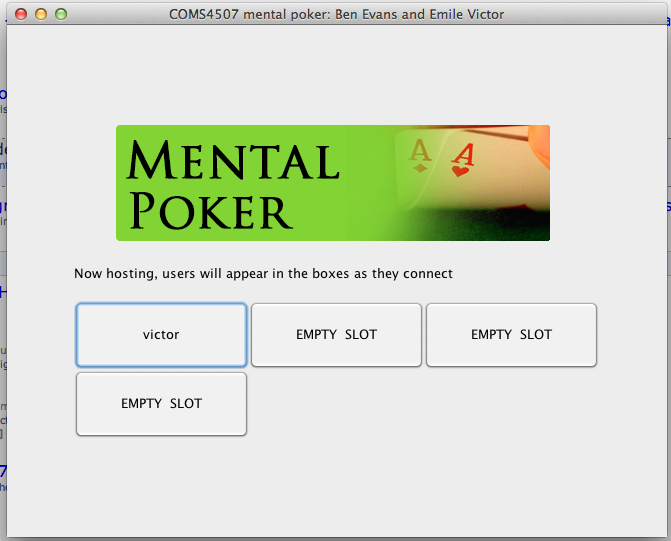
\includegraphics[bb=0 0 671 541,scale=0.55]{images/hostgame.png}
\end{figure}

\begin{figure}[h!]

\caption{The game search screen showing available games}
	\label{joinGame}
\centering
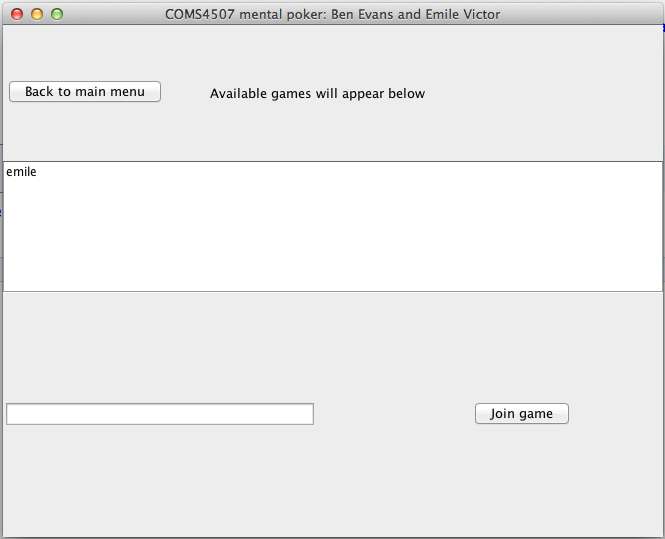
\includegraphics[bb=0 0 665 539,scale=0.55]{images/joinGame.png}
\end{figure}

\begin{figure}[h!]

\caption{Game Screen}
	\label{commCards}
\centering
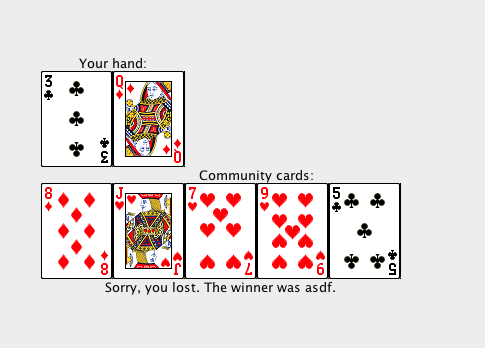
\includegraphics[bb=0 0 485 348,scale=0.7]{images/commCards.png}
\end{figure}



\end{document}  